\section{DeepSmith}

DeepSmith is our open source framework for compiler fuzzing~\footnote{DeepSmith available at: \emph{[URL redacted for double-blind review]}}. Figure~\ref{fig:deeptune} provides an overview of the system. Our compiler test case generation approach consists of two parts: first, a generative model for code samples inferred from open-source codes; the second, test case construction.

\cc{TODO: overview} We mine over a million lines of handwritten OpenCL code from GitHub, which we use to construct a corpus of representative programs. We learn a generative model over this corpus, using syntactic level language modeling. DeepSmith, our deep learning program generator, automatically and rapidly synthesizes an unbounded number of programs for fuzz testing compilers.


\subsection{Generative Model for Program Codes}

Generating test cases for compilers is hard because their inputs are highly structured. We employ state-of-the-art deep learning techniques to model program generation using unsupervised learning to build syntactic-level sequence models over source code. We extend prior work on synthetic program generation using Long Short-Term Memory (LSTM) networks~\cite{Cummins2017a}.

An initial seed corpus of 10k OpenCL kernels is mined from GitHub, using an oracle compiler (LLVM 3.9) to reject files that are not well-formed or do not contain instructions. The corpus is normalized using a custom LLVM pass to normalize syntactic choices --- identifier and function names.

A uniform code style is enforced to ensure consistent use of braces, whitespace. The preprocessed corpus is encoded using a hybrid token/character-level encoding~\cite{Cummins2017b}. \cc{More detail\ldots}

LSTM networks model the vocabulary distribution over the encoded corpus. We use a two layer LSTM network of 512 nodes each, trained using Stochastic Gradient Descent for 50 epochs, with an initial learning rate of 0.002 and decaying by a factor of a half every 5 epochs. % We use TensorFlow to implement the LSTM networks, with the entire generative model requiring less than 200 lines of Python, and is not specialized to OpenCL.

The trained network is sampled to generate new programs. The model is seeded with the start of a kernel (\texttt{\_\_kernel void}), and sampled token-by-token. A ``bracket depth'' counter is incremented or decremented upon production of \texttt{\{} or \texttt{\}} tokens respectively, and sampling terminates once the bracket depth reaches zero. The generated sequence of tokens are then concatenated and used as the generated program.

\cc{Add algorithm!}

\begin{figure}
  \centering
  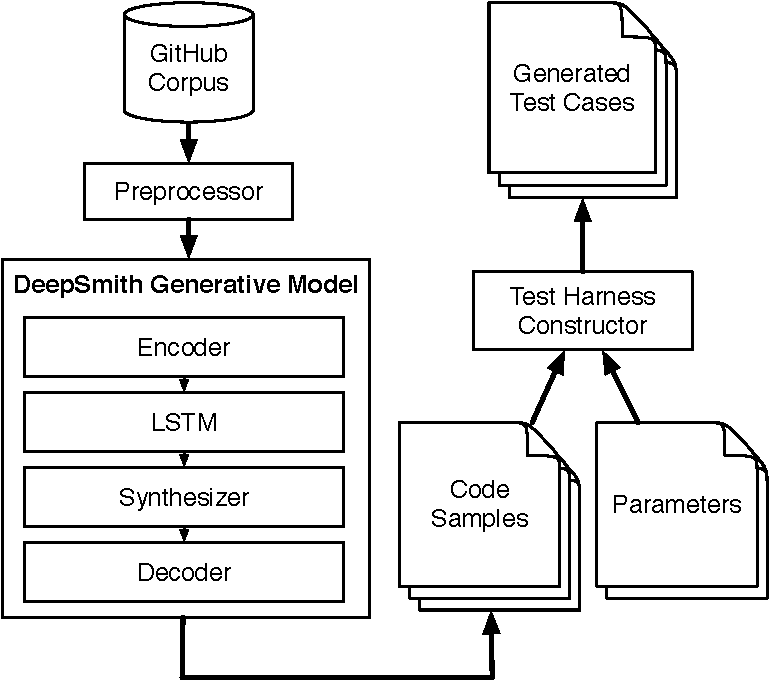
\includegraphics[width=.80\columnwidth]{img/deepsmith} %
  % \vspace{-2em}%
  \caption{%
    Test case generation. An corpus of programs from GitHub is used to seed a generative model for program code, which are parameterized to construct test cases. \cc{Add testbeds and comparison of outputs}%
  }%
  \label{fig:deeptune}
\end{figure}


\subsection{Test Case Execution}

\cc{reword - a single test harness accepts a string as input and generates input data}

OpenCL is an embedded compute kernel language, requiring host code to compile, execute, and transfer data between the host and device. For the purpose of compiler fuzzing, this requires a \emph{test harness} to run the generated OpenCL programs.

At first, we used the test harness of CLSmith. CLSmith kernels accept no inputs, and each thread computes the same value which is stored in a \texttt{ulong} buffer. The fixed function prototype means that they have a single re-usable test harness which may compile any CLSmith kernel, run it, and prints the output. We found this fixed harness to be too inflexible for our needs. This prototype is not a common OpenCL use case (only 5.6\% of GitHub kernels accept a single argument, and 0.2\% a single \texttt{ulong}).
% $ grep -E '^__global (.*)\* A$' github-arguments.txt | wc -l     -> 294
% $ grep '^__global ulong\* A$' ~/src/project_b/difftest/github-arguments.txt | wc -l     -> 10
To test a more expressive range of kernels, we created a test harness capable of driving arbitrary OpenCL kernels.

OpenCL kernels are executed concurrently one or more threads. We parameterize test harness generation with a single value $n$. For each program, we generate two test harnesses, one where $n=1$ (i.e. a single thread computing a single result) and one where $n = 2048$. For a given OpenCL kernel, we first parse the function prototype in order to determine the expected arguments. We then generate host data to feed to these arguments --- supporting scalars and arrays of all OpenCL primitive and vector types. Input arrays are generated of size $n$ and populated with values {$[1 \ldots n]$}; scalar values are given value $n$. We then enqueue the kernel on $n$ threads. The \emph{output} of a program is the values of all non-const arguments after kernel execution.

Since we do not guarantee that the generative model samples are well-formed, it may not be possible to parse the function signature. In this case, a ``compile-only'' stub is generated, which only compile the kernel, without generating input data or executing the compiled kernel.

We note that, unlike the generative model, this test harness construction is language-specific and the design stems domain knowledge. Still, it is a relatively simple procedure, consisting of a few hundred lines of Python.

% SELECT (SUM(compile_only) / (
% SELECT COUNT(*)
% FROM CLgenResults results
% INNER JOIN CLgenMetas meta ON results.id = meta.id
% WHERE cumtime < 48 * 3600
% )) * 100 as '% compile-only'
% FROM CLgenResults results
% INNER JOIN CLgenMetas meta ON results.id = meta.id
% INNER JOIN CLgenHarnesses harnesses on results.testcase_id = harnesses.id
% WHERE cumtime < 48 * 3600;
% 21.5\% of test cases are compile-only stubs.


\subsection{Test Case Execution}

\begin{figure}
	\centering %
	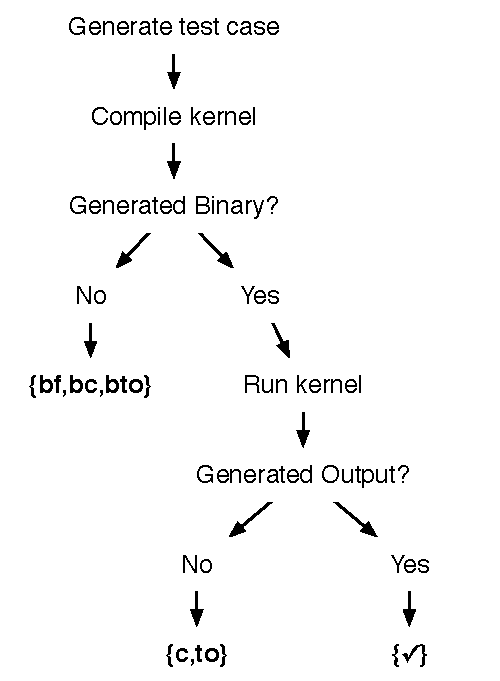
\includegraphics[width=.8\columnwidth]{img/test_process}%
	\caption{%
		Test case execution, and possible results. On each testbed, test case execution produces one of seven possible outcomes: \{bf,bc,bto,c,to,w,\cmark\}.%
	}%
	\label{fig:test-process} %
\end{figure}

% We classify the result of executing a test case into one of six classifications: build failure (\textbf{bf}), build crash (\textbf{bc}), runtime crash (\textbf{c}), or pass (\textbf{\cmark}). A \textbf{bf} occurs when compilation of a kernel fails, usually accompanied by an error message. A \textbf{bc} outcome occurs when the compiler crashes. A \textbf{c} outcome occurs when the program crashes during execution. The \textbf{bto} and \textbf{to} outcomes occur when the program compilation or execution time out, respectively.

\cc{TODO: Rewrite with only bc,bto outcomes, else voting heuristic}

Executing a test case on a testbed leads to one of six possible outcomes: \textbf{\{bf,bc,bto,c,to,\cmark\}}, illustrated in Figure~\ref{fig:test-process}.

A \emph{build failure} (\textbf{bf}) occurs when online compilation of the OpenCL kernel fails, usually accompanied by an error diagnostic. A \emph{build crash} (\textbf{bc}) or \emph{build timeout} (\textbf{bto}) outcome occurs if the compiler crashes or fails to produce a binary within 60 seconds, respectively. For compile-only test cases, a \emph{pass} (\textbf{\cmark}) is achieved if the compiler produces a binary. For test cases in which the kernel is executed, kernel execution leads to one of three potential outcomes: \emph{runtime crash} (\textbf{c}) if the program crashes, \emph{timeout} (\textbf{to}) if the kernel fails to terminate within 60 seconds, or \emph{pass} (\textbf{\cmark}) if the kernel terminates gracefully and computes an output.
%
%\begin{enumerate}
%	\item \emph{Build failure} (\textbf{bf}) Online compilation of the OpenCL kernel fails, usually accompanied by an error diagnostic.
%	\item \emph{Build crash} (\textbf{bc}) The compiler crashes during online compilation of the OpenCL kernel.
%	\item \emph{Build timeout} (\textbf{bto}) Online compilation of the OpenCL kernel exceeds the timeout of 60 seconds.
%	\item \emph{Runtime crash} (\textbf{c}) Compilation of the OpenCL kernel succeeds gracefully, but the program crashes during kernel execution.
%	\item \emph{Runtime timeout} (\textbf{to}) Compilation of the OpenCL kernel succeeds gracefully, but program execution exceeds the timeout of 60 second.
%	\item \textbf{\cmark} \emph{Completion} The program terminates gracefully and produces an output.
%\end{enumerate}

When evaluating the outcomes of test cases, \textbf{\{bc,bto\}} outcomes are of immediate interest, indicative of erroneous compiler behavior \cc{examples in Section~\ref{subsec:compile-time-defects}}. For all other outcomes, \emph{differential tests} are required to expose anomalous behavior.


\subsection{Voting Heuristics for Differential Testing}

As in prior work, voting on the output of programs across compilers has been used to circumvent the \emph{oracle problem} and detect miscompilations~\cite{McKeeman1998}.
% In~\cite{Lidbury2015a}, a testbed is determined to have produced a wrong code result for a kernel if there is a majority output of at least 3 among the \textbf{\cmark} results for the kernel, and the testbed yields a \textbf{\cmark} result that disagrees with the majority.
We extend this approach to describe not only miscompilations, but also anomalous build failures, crashes, and timeouts \cc{do we?}.

A majority outcome exists if, for for a particular test case ran on $n$ testbeds, at least $\ceil{\frac{2}{3}n}$ testbeds produce non-\textbf{\{bc,bto\}} results with the same outcome. We classify anomalous results with respect to the majority outcome for each test case.

A \emph{build failure} (\textbf{bf}), \emph{runtime crash} (\textbf{c}), or \emph{timeout}(\textbf{to}) result occurs if, for a given test case, the majority of testbeds produce an output, and a testbed yields compilation error, runtime crash, or timeout result.

A \emph{wrong-output} (\textbf{w}) occurs if, for a given test case, the majority of testbeds produce an output, at least $\ceil{\frac{2}{3}n}$ testbeds compute the same result, and a testbed yields a result which differs from this majority output. A \textbf{w} result is indicative of a \emph{miscompilation}, a particularly hard to detect class of bug in which the compiler silently emits the wrong code. CSmith is designed specifically to target this class of bug.


% Only 2.3\% of CLSmith programs with anomalous outputs are insensitive to optimization level.

%
%\begin{enumerate}
%	\item \textbf{w} \emph{Wrong code} Program terminates gracefully, but computes a result which differs from the majority output. For a DeepSmith result to be classified with \emph{wrong-code}, we require first that the program passes verification using GPUVerify~\cite{Betts2012}, and that a reference run with Oclgrind~\cite{Price2015} produces no warnings. \cc{Vote on compiler warnings, and optimization sensitivity. This means we way miss bugs which optimization level insensitive, though our experiences testing with CLSmith revealed only discovered 2 such cases}.
%	\item \textbf{bf} \emph{Build failure} Online compilation of OpenCL program fails, whereas the majority of testbeds produce a binary. \cc{TODO: with voting to exclude programs which rely on OpenCL 2.0 / compiler specific features}
%	\item \textbf{c} \emph{Runtime crash} One or more OpenCL API calls return an error status during the program execution, or the program crashes.
%	\item \textbf{to} \emph{Runtime timeout} Program execution exceeds the timeout of 60 second, whereas the majority of testbeds produce an output.
%\end{enumerate}


% \subsection{Design Trade-Offs}\label{subsec:discussions}
% Discussions?

\cc{TODO: compress and merge into heuristics discussion above:}

% \paragraph{Design Trade-Offs}
Our sequence-to-sequence approach to program generation greatly simplifies the implementation --- targeting a new language requires only a corpus of example programs and a test harness for generated codes. The generative model itself contains no language-specific code, and is implemented in less than 200 lines of Python --- a small fraction of that of prior approaches. The trade-off of this makes significantly reduces the cost of development, but we provide no guarantees on generated program correctness.

\paragraph{Undefined Behaviors} % aka. unambiguous observable behaviour
Differential testing on the output of a generated program requires that the program does not rely on undefined behavior. OpenCL doesn't have the rich tooling of C --- no CompCert and UBSan, there is much work to be done. GPUverify~\cite{Betts2012} and Oclgrind can catch some errors such as data races and out-of-bounds error checks, but as we have shown in Section~\ref{sec:motivation}, this tool is not without flaws. Compiler warnings are useful for obvious missteps (e.g. comparison between pointer and integer), but our approach does not rule out manual inspection. DeepSmith programs are easily interpretable --- they are generally short programs built on common language constructs, so this process is not as bad as it could be. We have not yet discovered an false-positive result which was not trivially detectable by automated filtering.

\paragraph{OpenCL Versions and Extensions} OpenCL is a fast evolving language, with six standard revisions in eight years. Vendor support for standard versions is inconsistent, as is the support for optional language extensions. Since we do not version the GitHub corpus on which we built the DeepSmith models, this has the potential to lead to false-positive results for programs which depend upon features which are not supported by a testbed. For example, not all testbeds support the optional \texttt{cl\_khr\_fp64} extension which provides support for double-precision floating point. We found that such results were trivially detectable through compiler error messages, and used to prevent false-positives for anomalous build failures.

\paragraph{Floating Points} The OpenCL specifications permit acceptable error bounds (ULP) for floating point operations and builtin functions. Some operations like addition, and multiplication are precise; divide permits a small error, and builtins vary widely. Thus two implementation may give different answers that both fit within the allowed ranges (and because errors propagate through operations it's hard to even describe the ULP on the final output). For this reason, CSmith, and by extension, CLSmith, do not support floating point operations. We believe this restriction to be artificially limiting, since floating point computations are dominant in the common uses of OpenCL --- %
% $ ls | xargs grep -E -l '(float|double)' -- | wc -l  # 2245
48\% of GitHub kernels use floating points. At the moment, we simply print floating values using \texttt{printf()} rounding. This will hide small rounding errors. Larger errors prevent us from difftesting on the output since no output majority will be possible. Given knowledge about hardware imprecision, it would be possible to compute an acceptable error threshold for floating point results based on dynamic profiling.

\paragraph{Divide-by zero} \cc{TODO} The hardest false-positive to prevent was division by zero and related mathematical functions which require non-zero values. In all cases we discovered these can be detected by simply changing the input values and checking to see if the output remains anomalous.

% Section 7.4 of OpenCL 1.2 spec.

\paragraph{Small, Human-like Test Cases} Random token / grammar enumeration has previously been used to target parsers and lexers. CSmith creates huge, ``ugly'' programs with the intention of deliberately targeting bugs in IR transformations --- the middle-end.

One might expect our approach --- generating small test cases in the style of handwritten programs --- is perhaps less likely to find bugs than CSmith, which generates huge, ``ugly'' programs pairing infrequently used language features. DeepSmith rarely generates large OpenCL kernels because humans rarely write them. A code which is more likely to be written by a human is also more likely to be included in the compiler test suites, \cc{hmm what do we do about this}